\documentclass[a4paper,ngerman]{scrartcl}

\usepackage{amsmath}
\usepackage{amsfonts}
\usepackage{amssymb}
\usepackage[utf8]{inputenc}
\usepackage{graphicx}
\usepackage[ngerman]{babel}
\usepackage{hyperref}
\usepackage{float}
\usepackage{caption}
\usepackage{subcaption}
\usepackage{multirow}  %for tables
\usepackage{icomma} % Handle german comma as decimal point in numbers
\usepackage{units,siunitx} % Write units with correct spacing
\usepackage{upgreek} % provide non-italic greek letters
\usepackage{url}
\usepackage{hepnames} % hier gibt es symbole fuer unterschiedliche elementarteilchen, aber dieses paket gibts nicht im poolraum

%\usepackage{subfig}

% Formatting of table & figure captions
\captionsetup{font={sf,footnotesize},labelfont=bf,textfont=sl,skip=6pt}

\sisetup{locale = DE, % use "," as decimal point instead of "."
  exponent-product={\cdot},% used \cdot in front of 10^x
  separate-uncertainty} % give out uncertainty with \pm instead of in brackets

\setlength{\abovecaptionskip}{6pt}
\setlength{\belowcaptionskip}{0pt}

\title{Elementarteilchen 2\\Vorbereitung}
\date{\today}
\author{Michel Rausch, Michael Eliachevitch}

\begin{document}

\maketitle
\tableofcontents
\newpage

\section{Einleitung}

\section{Das DELPHI Experiment am LEP}
\label{sec:delphi}

\begin{figure}
\centering
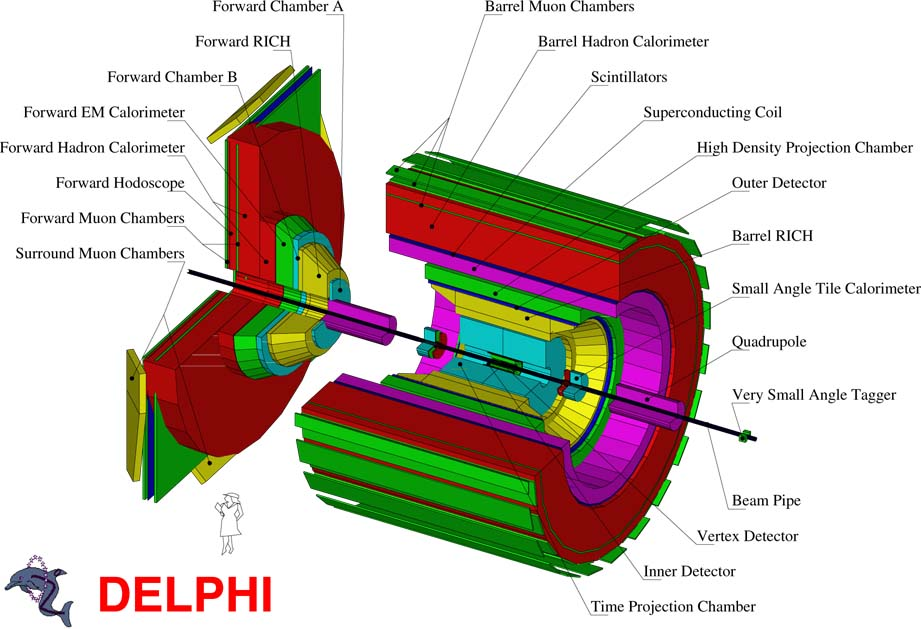
\includegraphics[width=\textwidth]{abbildungen/delphi_big.png}
\caption{\textbf{Aufbau des DELPHI-Detektors mit einer sichtbaren Endkappe [\ref{ref:hands-on}].} 
Die Bestandteile des Detektors sind farblich gekennzeichnet und benannt.
Links ist eine der beiden Endkappen zu sehen, die andere wurde zur Übersichtlichkeit ausgeblendet.
Rechts im Bild ist der zylindrische zentrale Teil mit Strahlengang gezeigt. 
}
\label{fig:delphi_big}
\end{figure}





\begin{figure}
\centering
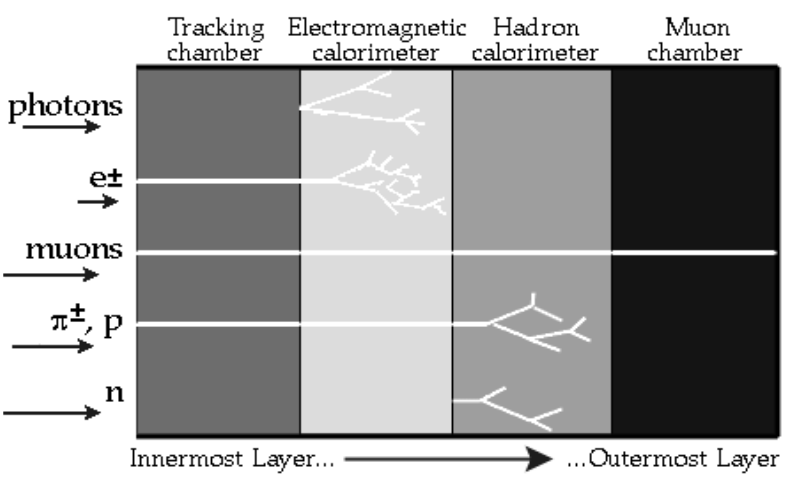
\includegraphics[width=0.7\textwidth]{abbildungen/delphi_schichten.png}
\caption{\textbf{Übersicht der Signaturen nachweisbarer Teilchen in den Subdetektoren [\ref{ref:BB}].} 
}
\label{fig:delphi_schichten}
\end{figure}


%\section{Mögliche Zerfälle und Bestimmung der Zerfallsbreiten und Kopplungskonstanten}
\section{Theoretische Betrachtung unterschiedlicher Zerfälle}
\label{sec:zerfaelle}

Wie bereits in Kapitel~\ref{sec:delphi} angesprochen, wurden im LEP \Pelectron-\APelectron-Paare zur Kollision gebracht, wobei gegen Ende Schwerpunktsenergien von über 200\,Gev~\ref{ref:cernlep} erreicht wurden,
womit neue Teilchen erzeugt werden konnten.
Dabei konnten neue Teilchen entstehen, 
solange diese die Erhaltungssätze des Standardmodells nicht verletzen 
und deren Energie nicht die Schwerpunktsenergie der Kollision übersteigt.
Aufgrund der Erhaltung der elektrischen Ladung und der Farbladung, 
die beide in der Summe bei dem \Pelectron-\APelectron-Paar null sind,
entstand bei einer Kollision immer zuerst eines der beiden neutralen Eichbosonen,
nämlich entweder ein Photon oder ein \PZzero-Boson,
welches eine Ruhemasse von 91\,GeV~\ref{ref:BB} besitzt.
Beides sind virtuelle Teilchen, die schnell in weitere Teilchen zerfallen,
weshalb aufgrund der Unschärferelation die Masse des virtuellen
Teilchens die Energieerhaltung auch verletzen kann.
Wir werden in diesem Versuch die Zerfälle des \PZzero-Bosons betrachten.\\

Die virtuellen Eichbosonen können in Leptonen-Antileptonen- oder auch 
Quark-Antiquark-Paare unterschiedlicher Teilchenfamilien zerfallen. 
Die Teilchen der schwereren Teilchenfamilien sind instabil und zerfallen weiter in leichtere Teilchen.
Bei Quarks ist zu beachten, dass diese nicht frei existieren können,
da die starke Kernkraft bei zunehmendem Abstand zunimmt.
Durch die große potentielle Energie bilden sich neue Quark-Antiquark-Paare,
bis am Ende nur noch gebundene Zustände Quarks vorhanden sind. 
Dabei handelt es sich um 
Mesonen aus Quark und Antiquark mit entgegengesetzter Farbladung und um Hadronen aus 3 Quarks,
in denen jede Farbladung vorhanden ist. 
Dabei entstehen sogenannte Jets. 
Es gibt immer mindestens zwei davon, da das \PZzero zuerst in ein Quark-Antiquark-Paar zerfällt. 
Dann spricht man von 2-Jets.
Oft gibt es auch drei Jets, sogenannte 3-Jets, wobei der dritte Jet durch Gluonabstrahlung entsteht,
welches wie die Quarks eine Farbladung hat und damit der starken Wechselwirkung unterliegt und folglich ebenfalls Jets erzeugt.
Die Entstehung eines 3-Jets aus dem Zerfall eines in einer \Pelectron-\APelectron-Kollision entstandenen \PZzero-Bosons ist 
in dem Feynmandiagramm in Abbildung ... gezeigt.
Da das Gluon mit der starken Kraft an das Quark koppelt, ist die Wahrscheinlichkeit eines 3-Jets durch die 
Kopplungskonstante der starken Kernkraft gegeben.

\begin{figure}[tbh!]
  \centering
  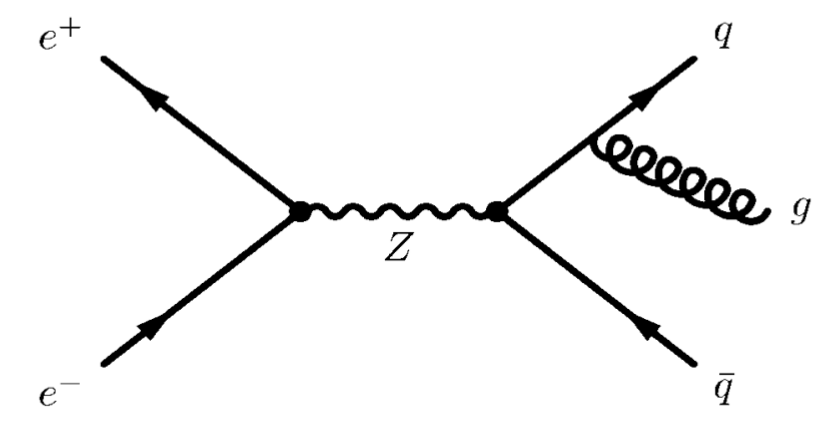
\includegraphics[width=0.7\textwidth]{abbildungen/3jet_feyn.png}
  \caption{Entstehung eines 3-Jets im LEP.\\ Bei der Kollision von Positron und Elektron bildet sich ein virtuelles \PZzero, welches in ein Quark-Antiquark-Paar zerfällt, die beide einen Jet erzeugen. Durch die Abspaltung eines Gluons, deren Wahrscheinlichkeit durch die Kopplungsstärke der starken Kernkraft gegeben ist, bildet sich ein dritter Jet.}
  \label{fig:3jet}
\end{figure}










\section{Das Scannen von Ereignissen mit "`Fireworks"' und Beispielzerfälle}
\label{sec:scannen}

\section{Quellen}
\begin{enumerate}
\item Blaues Buch \label{ref:BB}
\item \url{http://home.web.cern.ch/about/accelerators/large-electron-positron-collider} (\today) \label{ref:cernlep}
% Quelle fuer PDG-Angaben: (noch nicht genutzt, daher auskommentiert)
% \item K.A. Olive et al. (Particle Data Group), Chin. Phys. C, 38, 090001 (2014). \label{ref:pdg14}
\item \url{http://hands-on-cern.physto.se/hoc_v21en/index.html} (\today)\label{ref:hands-on}
\end{enumerate}



\end{document}
